\section{Introduction}
\label{sec:intro}

Ridership on many public transit systems in the US has been on the decline despite significant investments \cite{William01}. Any improvements in efficient scheduling of buses and optimal planning of bus routes, with the ultimate goal of improving rider experience, is vital to increasing adoption of public transit systems and keeping them relevant. To this end, real-time data collection of crowd densities of buses can be used to develop data-driven approaches for improving resource efficiency and rider experience. Combined with existing real-time bus tracking, this data will enable riders to check not just if and when a bus is approaching, but also whether it is fully occupied. For transit operators, the data could prove to be valuable in analyzing crowd transit patterns and employ dynamic bus scheduling techniques. In the longer term, it will also allow them to assess optimal bus routes to improve ridership given the limited amount of resources. \\

Some transit agencies have already been using Automatic Passenger Counter (APC) systems that involve some sort of sensors (treadle mats, IR sensors, etc.) installed at the entry and exit doors which count number of people boarding and alighting at any stop. While these techniques provide highly accurate counts, they are usually expensive, or usually involve complicated installation and/or  regular maintenance. In contrast, Bluetooth or Wi-Fi sensors are relatively cheap and easier to install, and with the solutions we explore in this paper, only one sensor needs to be installed. If precise count is not required, which we believe is the case for the applications we mentioned, these sensors can provide a simpler and cheaper alternative to the APCs. \\

A recent study on mobile device ownership \cite{PewSurvey01} finds that 77\% of Americans own a smartphone (and not just a cellphone) of some kind, which shows how ubiquitous these devices have become. With the reasonable assumption that every smartphone comes with Wi-Fi and Bluetooth sensors, it opens up potential opportunities to use these devices as proxies and count them to get a good approximation of crowd density. In this paper, we present techniques that use both Wi-Fi and Bluetooth signals to detect presence (and the degree of presence) of these devices. With Bluetooth, we use bluetooth discovery mechanism to scan for nearby devices in regular intervals. In case of Wi-Fi, we passively monitor for so-called probe request frames that are sent out by the devices in regular intervals. We show that although both these techniques have their limitations and, consequently, are imperfect, they can provide a good approximation for the relative changes in crowd density as people board and alight at bus stops. \\

The remainder of the paper is structured as follows. In the next section, we look at previous work that is relevant to the problem. In section \ref{sec:datacollection}, we talk about how we went about data collection and getting the ground truth for our experiments. Thereafter, in sections \ref{sec:bluetooth} and \ref{sec:wifi}, we present our experimental methodologies for estimating crowd density using Bluetooth and Wi-Fi data respectively and the results of these experiments. We then discuss the feasibility and limitations of our approaches in section \ref{sec:discussion}, and finally we conclude the paper with a short summary and future work in section \ref{sec:conclusion}. \\


\section{Related Work}
Indoor localization using wireless signals has been thoroughly studied in the past couple of decades. One is tempted to apply these techniques to the problem of crowd density detection. However, even the best of the accurate localization techniques \cite{ActiveLoc01} need devices being localized to be actively sending packets, which is not a reasonable expectation in our scenario. While there are some passive localization techniques that take advantage of reflections of wireless signals caused by disturbances in environments caused by human presence \cite{PassiveLoc01}, these currently cannot deal with more than one person at a time. Moreover, all these techniques need multiple access points deployed which cannot be a better alternative to APCs we mentioned in section \ref{sec:intro}. \\

When it comes to collecting ridership data using wireless signals, there has been lot of work that uses probe requests to achieve this with varying degrees of success \cite{BusCrowd01, BusCrowd02, BusCrowd03, BusCrowd04}. While Thongtat et al. \cite{BusCrowd01} explore the Bluetooth technique, they discard it right away as unusable which we show is not the case. All the others use very similar Wi-Fi techniques that we describe in this paper to use probe requests for crowd density estimation. (\textbf{Note to Aaron}: Found these papers only couple of days ago \textbf{:(} - for the purpose of this report, I assumed that these papers did not exist.) None of these papers address for the issue of mac-address randomization (which we will look into in detail in section \ref{sec:wifi}) that challenges their dependency on the uniqueness of the MAC addresses across the probe packets received from the same device. 


\section{Data Collection \& Ground Truth}
\label{sec:datacollection}
We performed our experiments on MTS public transit buses, on one of the popular bus routes (called UCSD Superloop) that is widely used by students of UC San Diego. For Bluetooth data, we used an android phone with an app called Bluetana, that uses Android bluetooth discovery mechanism to scan for devices every few seconds. This data is then uploaded to our backend server over cellular connection for later analyses. For Wi-Fi data, we use the WireShark packet capture software in monitor mode running on a MacBook Pro 2015 laptop. The software capture all the traffic in the area, irrespective of the source and destination of the packets and the data collected from each packet includes information belonging to each layer of the TCP/IP stack. We only collected the traffic in 2.4GHz range, we believe this will be enough for preliminary analysis as majority of the Wi-Fi traffic still uses this range. \\


We have conducted two experiments on different days. Each experiment starts at a bus stop and ends after two loops once bus reaches the same stop for the second time. We only present results from one of the experiments in this paper, but results of our approaches in both experiments are similar. To maximize reachability of the sensors from all the devices in the front and the back of the bus, we placed the sensors at halfway point in the bus. The buses we used were equipped with APC (Automatic Passenger Counter) systems that record number of passengers boarded and alighted at each bus stop. We received this data for our experiments from MTS support team, which we used as ground truth to analyze our results. 


\section{Bluetooth}
\label{sec:bluetooth}

\subsection{Methodology}
Most devices today come with inbuilt support for bluetooth technology that enables peer-to-peer wireless communications. These communications occur over short-range networks called piconets. For consumer devices, this range usually goes up to 10 meters, which makes it really suited for our scenario where all the devices of interest (i.e., inside the bus) will be well within this range and there will be less external noise to deal with. (In this respect, it has an advantage over Wi-Fi, as Wi-Fi has a larger range and so it is more prone to  noise from external devices). \\

The data we collected contains the records for all the devices that are discovered in each scan. Each record contains the time stamp, MAC address of the discovered device, signal strength (RSSI), device type (classic or low-energy) and GPS location among others. We use MAC address to uniquely identify a device and cluster all the observed records for the same device. While bluetooth devices have started implementing MAC address randomization, it is not so prevalent as in the case of Wi-Fi (which we discuss in detail in section \ref{sec:wifi}), so we assume that it won't affect our analyses. Once we cluster the observed records of the devices, the next step is to filter out external devices. Here, we take advantage of the insight that since the bus is constantly moving, external devices will go out of range soon enough and consequently, will only be visible for shorter time periods. After eliminating external devices using this insight, we count number of remaining devices that are present at each second of the trip and present it as our estimate for the crowd density. (We count a device as "present" for all the seconds between first and last observations of the device).

\subsection{Results}

\begin{figure}[!t]
\centering
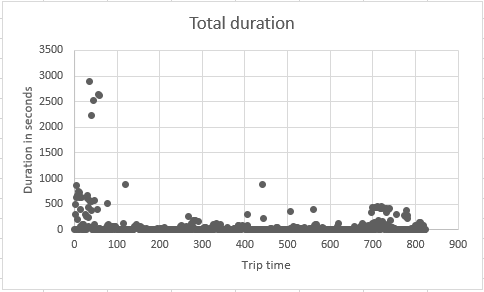
\includegraphics[width=0.5\textwidth]{ble_device_durations.png}
\caption{Bluetooth: Lengths of duration for observed Bluetooth devices. Most of the devices were observed only for up to two or three minutes, which means they are external. Others in the 200 to 1000 second range correspond to the legitimate traffic from devices inside the bus, while few data points over 2500 seconds likely correspond to external devices picked up in the second loop of the trip.}
\label{fig:btdurations}
\end{figure}

\begin{figure}[!t]
\centering
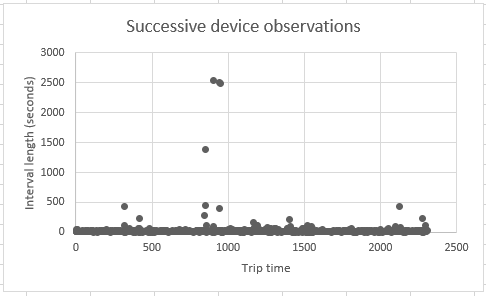
\includegraphics[width=0.5\textwidth]{ble_interval_lengths.png}
\caption{Bluetooth: Length of intervals between successive observations of devices that were observed more than once. It shows that most devices, if they continue to be around, are detected again within a minute.}
\label{fig:btintervals}
\end{figure}

\begin{figure}[!t]
\centering
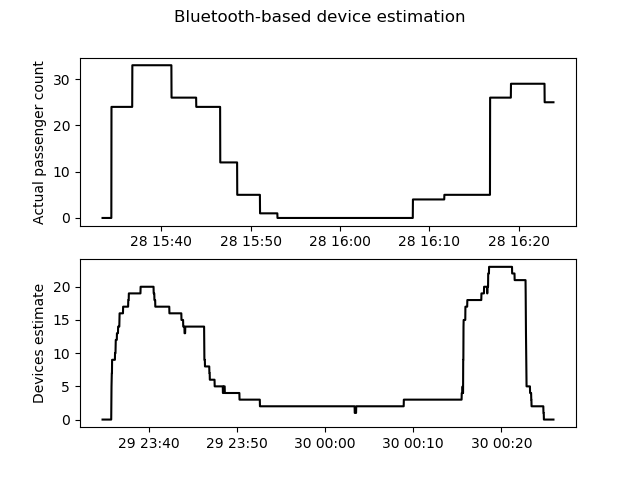
\includegraphics[width=0.5\textwidth]{ble_devices_estimate.png}
\caption{Bluetooth: The top plot shows the ground truth passenger count while the bottom one presents our estimates based on bluetooth data.}
\label{fig:btestimate}
\end{figure}

We show some of our observations and results for bluetooth data in Figures \ref{fig:btdurations}, \ref{fig:btintervals} and \ref{fig:btestimate}. To filter out external traffic, we used the 3-minute cutoff for the total observation duration for each device, as explained in Figure \ref{fig:btdurations}. Figure \ref{fig:btintervals} shows that any device that is detected more than once has less that 1 minute period between successive detections. We used this observation to eliminate external traffic that persisted for more than 3 minutes (e.g., traffic picked up on the second loop) but did not have the number of detections that is proportional to the length of observed duration. Our final results are presented in Figure \ref{fig:btestimate}. While the estimate is inaccurate in terms of the actual count (as expected) i.e., maximum number of devices estimated is 20 while actual passenger count goes up to 30, it nevertheless shows a good correlation with the ground truth data. Note that although the estimate peaks seem narrower compared to original ones, it is because of slight difference in time axes of both the plots (You can look at the seconds to correlate).


\section{Wi-Fi}
\label{sec:wifi}

\subsection{Methodology}
One of the defining features of a smartphone is the ability to connect to internet through Wi-Fi. In addition to the actual data frames used to transfer data between devices and access points, Wi-Fi uses different types of management frames to search for and manage connections to these access points. In our scenario, we only considered the management frames from the data we collected as most buses do not have Wi-Fi access points and consequently, no data traffic originates from devices inside the bus - this also eliminates lot of external traffic we otherwise have to deal with. Within management frames, we were only interested in a specific type called probe request frames, that are used by devices to inquire for nearby access points. Since most of the devices on the bus will be in disassociated state (i.e., not actively connected to any access point), most of the traffic from these devices will be in form of probe requests sent in regular intervals. We use the probe requests from the captured Wi-Fi traffic to track the presence of these devices and estimate their count.  \\

Probe requests, like any other Wi-Fi frames, carry MAC address information which can be used to identify devices. Since probe
requests continuously broadcast at a semi-constant rate they make tracking trivial. To address privacy concerns arising out of this, some modern mobile devices make use of temporary, randomized MAC addresses that are distinct from their true global address. When probe requests are sent out, they use a randomized pseudonym MAC address that is changed periodically - and the periodicity varies across different vendors. This makes grouping the probe requests sent by the same device nearly impossible as we lost the only key that can uniquely identify the device. There were studies that show that MAC address randomization itself is actually not enough to avoid tracking, as randomization itself could be imperfect and probe requests usually contain huge amount of other information (like sequence numbers, tags, etc.) that could be used as a signature for the device \cite{MacRandomization01, MacRandomization02}. In this paper though, we limited ourselves to the traffic from the devices that still use their true MAC addresses (which account for almost 50\% of the observed devices in our data). Our idea is that while the filtered out traffic would surely hurt our ability to accurately predict the exact number of devices, it would still not affect the trend, which is what we were interested in. We do however explored the possibility of building up device signatures to overcome MAC address randomization, and we treat this as future work. \\

The first step in processing the data we captured is filtering for probe packets, which was trivial by using 802.11 management type field. Next, we removed all the packets with randomized MAC addresses. We considered a MAC address to be real if we see it more than once in the data, and once a real MAC address is found, the assumption is that the device associated with this address would send all its packets with the same MAC address. Thereafter, we grouped the packets based on their MAC addresses. To eliminate the clusters associated with external devices, we used the same intuition, as with Bluetooth devices in section \ref{sec:bluetooth}, that these clusters will only last for shorter periods of time. With Bluetooth, figuring out this time threshold was made simpler by less external noise and the regularity of the intervals between successive device observations. With Wi-Fi however, there was significantly more noise because of its larger range, and the probe requests vary widely in terms of time between successive appearances, as the periodicity varies across different manufacturers. The problem is worsened by frequently missed or malformed packets, which seems to be a common case. Based on our observations, we arrived at a heuristic to classify the probe packet clusters from a device as external traffic if they didn't last longer (i.e., the time between first and last probe requests) than 3 minutes, or if they persisted more than 3 minutes and the length of any interval between successive probe packets in the cluster does not exceed 2 minutes. We discuss the results of our approach in the next section. \\

\subsection{Results}

Figures \ref{fig:wifidurations} and \ref{fig:wifiintervals} show scatter plots for lengths of observed duration of each device and intervals between successive probe packets coming from the same devices respectively. Compared to similar plots for Bluetooth (Figures \ref{fig:btdurations} and \ref{fig:btintervals}), these plots are much more scattered due to more noise from external traffic and variance in probe request intervals. These features make the simple thresholds we used in Bluetooth unusable for Wi-Fi. First, we filter out external traffic based on a threshold for duration, which would be higher compared to Bluetooth as external devices stay longer in Wi-Fi's larger capture range. After this step, the external traffic that is not filtered out would be the devices captured in the second loop of the trip (the top-left corner of each figure shows this noisy traffic captured from such external devices). To eliminate these, we run through the length of intervals between successive probe requests and eliminate the devices where this crossed a certain threshold. From figure \ref{fig:wifiintervals}, 2 minutes seemed to cover majority of such intervals which we will use for this threshold. \\

Our estimate for crowd density using this approach is shown in Figure \ref{fig:wifiestimate}. While the first and last peaks correlate well (note that the estimate peaks seem to be a bit narrower because of the axes synchronization issue as with Figure \ref{fig:btestimate}), there is an unexpected peak that doesn't not correspond to any crowd on the bus. This was because of the long 3-minute wait at a major bus stop where the operator took a small break. In this case, there is no mobility and our algorithm could not differentiate between outside traffic vs inside traffic corresponding to a crowd getting on at a bus stop and getting off at a different one 3 minutes later. In such cases, the geo-location information of the bus could prove to be useful for excluding such false data generated when the bus is fixed to a spot for a long time. We talk more about benefits of adding location data in the discussion section. Similar to Bluetooth, while the exact count is not matched, the figure shows that the a good approximation of the trend can be achieved, and this despite discarding half of the data due to MAC address randomization.

\begin{figure}[!t]
\centering
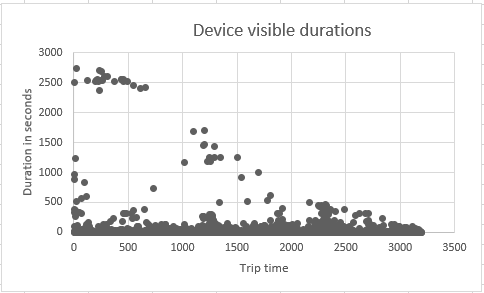
\includegraphics[width=0.5\textwidth]{wifi_device_durations.png}
\caption{Wi-Fi: Lengths of duration for observed Wi-Fi devices. Compared to Bluetooth, the data is more scattered as there is more external noise due arguably to larger range of captured Wi-Fi signals.}
\label{fig:wifidurations}
\end{figure}

\begin{figure}[!t]
\centering
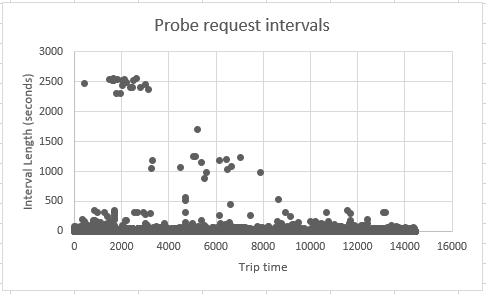
\includegraphics[width=0.5\textwidth]{wifi_interval_length.png}
\caption{Wi-Fi: Length of intervals between successive probe requests associated with the same devices. Compared to Bluetooth, the data is more scattered due to high variance in periodicity of probe requests across manufacturers and frequent packet misses in transmission.}
\label{fig:wifiintervals}
\end{figure}

\begin{figure}[!t]
\centering
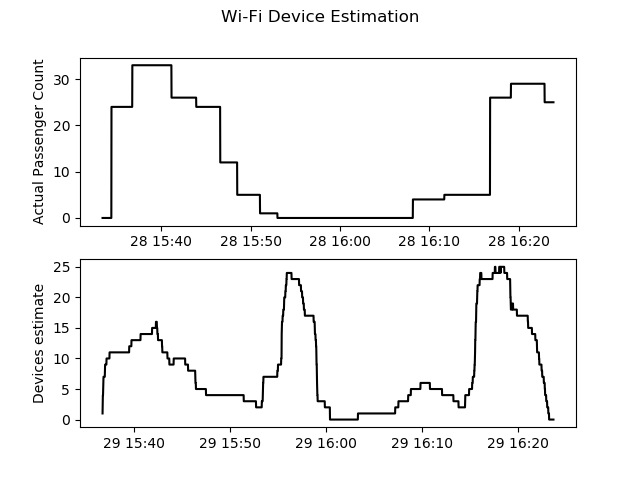
\includegraphics[width=0.5\textwidth]{wifi_devices_estimate.png}
\caption{Wi-Fi: The top plot shows the ground truth passenger count while the bottom one presents our estimates based on Wi-Fi data. The unexpected peak in the middle corresponds to the long wait (more than 3 minutes) at a major bus stop.}
\label{fig:wifiestimate}
\end{figure}


\section{Discussion}
\label{sec:discussion}

Our results show that, with the current state of Bluetooth and Wi-Fi data, both of them can provide good approximations to the actual crowd patterns with some simple heuristics applied to the raw data to reduce noise. Improvements can be made to the techniques used in both approaches to achieve better results in terms of better thresholds used for noise reduction but it should be understood that assessment of the exact count of the crowd could never be achieved due to inherent limitations of these approaches such as the inaccuracy of the assumption that every person uses exactly one device or not all devices will have their Bluetooth or Wi-Fi turned on at all times. As MAC address randomization becomes more common, which it is bound to be sooner or later, both these approaches will suffer as they only work on traffic with real MAC address. Wi-Fi approach offers potential opportunities to overcome the MAC address randomization issue, specifically with device signature techniques described by Vanhoef et al.\cite{MacRandomization02}. \\

One extra addition that could improve our techniques for noise reduction is the  geo-location data using GPS. This data combined with the time stamps could enable us to estimate the the times when the bus stops at bus stops or traffic signals. These stops usually go against our fundamental assumption that the bus is always moving, and so introduce the data that eludes techniques implemented with such assumption. Factoring in this knowledge could enhance our techniques that could let us avoid bad results like the unexpected peak we saw in Figure \ref{fig:wifiestimate}. We would like to note that we do collect this data as a part of our bluetooth data collection, however we haven't used it to improve our techniques as described above. We leave this to future work.


\section{Conclusion}
\label{sec:conclusion}

We aim to improve efficiency and rider experience of public transportation through data-driven approaches by collecting the real-time crowd density estimation in the buses. To this end, we evaluated the feasibility of using Wi-Fi and Bluetooth traffic originating from the devices in a bus to estimate the crowd, as they provide inexpensive and simpler alternatives to the problem compared to APCs. In this paper, we proposed simple techniques for noise reduction and device estimation using the collected Wi-Fi and Bluetooth data. We evaluated the accuracy of these approaches by comparing the results with the ground truth data of the experiments we performed on MTS buses in San Diego. We showed that while these approaches are not perfect, they can provide good approximations to changing crowd density in buses as riders board and alight them at bus stops. We concluded with a discussion on the limitations of these approaches and some enhancements which we left to future work.



\begin{acks}
  We would like to thank the San Diego MTS corp. (\href{https://www.sdmts.com/}{https://www.sdmts.com/}) for allowing us to perform experiments on their buses and more importantly, for providing the ground truth ridership data to evaluate accuracy of our solutions.
\end{acks}